\documentclass[../main.tex]{subfiles}
\begin{document}
%=========================================================
% TĐ_PBT_IQA_HK1_Tuan16_CacSoTrongPhamVi100_SoTronChuc
% Phiếu bài tập Toán tư duy cấp độ A
% Chủ đề CÁC SỐ TRONG PHẠM VI 100. SỐ TRÒN CHỤC (Buổi 1, Buổi 2)
% Soạn theo mẫu (\hktuan, bt, listEX)
% Hình đặt trong thư mục Hinh_Tuan16_PBT/ (cùng cấp với file này), tên hình có tiền tố t16_
% Đường dẫn tính từ thư mục của main.tex khi biên dịch main.tex
\graphicspath{{Hinh_Tuan16_PBT/}{Data_PhieuBaiTap_HK0/Hinh_Tuan16_PBT/}}
%=========================================================

%---------- Lệnh dùng riêng cho phiếu ----------
% Chèn hình căn giữa, dính liền với đề bài phía trên (không bị tách trang)
% Tham số tùy chọn = chiều cao tối đa của hình (mặc định 8cm); hình không rộng quá khổ giấy
\providecommand{\TThinh}{}\renewcommand{\TThinh}[2][8cm]{\par\nopagebreak\vspace{2pt}\nopagebreak{\centering\includegraphics[height=#1,width=\linewidth,keepaspectratio]{#2}\par}\vspace{2pt}}
% Chỗ chấm điền
\providecommand{\TTcham}[1][3cm]{\makebox[#1]{\dotfill}}
% Dòng thông tin học sinh
\providecommand{\TTthongtin}{%
  \noindent\begin{tabular}{|p{7.6cm}|p{4cm}|p{4cm}|}
    \hline
    \textbf{Họ và Tên HS:}\dotfill & \textbf{Lớp:}\dotfill & \textbf{Ngày:}\dotfill \\
    \hline
  \end{tabular}\par\medskip}
% Đánh lại số bài từ 1 cho buổi 2 (chỉ khi môi trường bt có bộ đếm tên bt)
\makeatletter
\providecommand{\TTdatlaibai}{\@ifundefined{c@bt}{}{\setcounter{bt}{0}}}
\makeatother
% Que tính: \TTbo{n} vẽ n bó một chục, \TTle{n} vẽ n que lẻ
\providecommand{\TTbo}{}\renewcommand{\TTbo}[1]{\foreach \i in {1,...,#1}{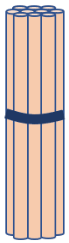
\includegraphics[height=1.6cm]{t16_image7.png}\hspace{1pt}}}
\providecommand{\TTle}{}\renewcommand{\TTle}[1]{\foreach \i in {1,...,#1}{
\includegraphics[height=1.6cm]{t16_image8.png}\hspace{3pt}}}
% Số để khoanh, cách đều nhau
\providecommand{\TTso}{}\renewcommand{\TTso}[1]{\makebox[1.5cm]{\textbf{#1}}}

%%%%%%%%%%%%%%%%%%%%%%%%%%%%%%%%%%%%%%%%%%%%%%%%%%%%%%%%%%
%                       BUỔI 1
%%%%%%%%%%%%%%%%%%%%%%%%%%%%%%%%%%%%%%%%%%%%%%%%%%%%%%%%%%
%\setcounter{section}{3} % không chỉnh sửa
\hktuan{1}{16}
\par\medskip % xuống dòng: tiêu đề không nằm chung dòng với khung HK1 - Tuần 16
{\centering
        {\color{mauchinh!120}\bfseries\Large PHIẾU BÀI TẬP TOÁN TƯ DUY CẤP ĐỘ A}\\[3pt]
        {\color{mauchinh!120}\bfseries\Large CHỦ ĐỀ: CÁC SỐ TRONG PHẠM VI 100.\\[2pt] SỐ TRÒN CHỤC (BUỔI 1)}\par}
\vspace{6pt}
\TTthongtin

\begin{bt}
    Đếm và điền số vào chỗ trống.
    \TThinh[4.2cm]{t16_image1.png}
    \TThinh[4.4cm]{t16_image2.png}
    \TThinh[4.6cm]{t16_image3.png}
    \TThinh[5cm]{t16_image4.png}
    \TThinh[7cm]{t16_image5.png}
\end{bt}

\begin{bt}
    Nối với số đúng.
    \TThinh[8cm]{t16_image6.png}
\end{bt}

\begin{bt}
    Viết số tương ứng với số lượng que tính.
    \par\nopagebreak\vspace{4pt}\nopagebreak{\centering
        \renewcommand{\arraystretch}{1.2}
        \begin{tabular}{|>{\centering\arraybackslash}m{6.2cm}|>{\centering\arraybackslash}m{5.2cm}|>{\centering\arraybackslash}m{3cm}|}
            \hline
            \TTbo{4} & \TTle{4} & \textbf{44} \\ \hline
            \TTbo{6} & \TTle{6} & \\ \hline
            \TTbo{3} & \TTle{9} & \\ \hline
            \TTbo{7} & \TTle{4} & \\ \hline
            \TTbo{8} & \TTle{9} & \\ \hline
            \TTbo{6} & \TTle{6} & \\ \hline
            \TTbo{9} & \TTle{2} & \\ \hline
        \end{tabular}\par}
\end{bt}

\begin{bt}
    Điền số thích hợp vào chỗ trống.
    \TThinh[8cm]{t16_image9.png}
\end{bt}

\begin{bt}
    Điền số thích hợp vào chỗ trống.
    \par\nopagebreak\vspace{4pt}\nopagebreak{\centering
        \renewcommand{\arraystretch}{1.6}
        \begin{tabular}{|>{\centering\arraybackslash}p{2.2cm}|>{\centering\arraybackslash}p{2.8cm}|>{\centering\arraybackslash}p{2.8cm}|>{\centering\arraybackslash}p{5.5cm}|}
            \hline
            \textbf{Số} & \textbf{Hàng chục} & \textbf{Hàng đơn vị} & \textbf{Cách đọc} \\ \hline
            43 & & & \\ \hline
             & 5 & 7 & \\ \hline
             & & & Bảy mươi sáu \\ \hline
            98 & & & \\ \hline
            27 & & & \\ \hline
             & & & Sáu mươi chín \\ \hline
             & 7 & 2 & \\ \hline
        \end{tabular}\par}
\end{bt}

\begin{bt}
    Nối số với cách đọc đúng.
    \TThinh[7cm]{t16_image10.png}
\end{bt}

\begin{bt}
    Điền số còn thiếu vào chỗ trống.
    \TThinh[8cm]{t16_image11.png}
\end{bt}

\begin{bt}
    Tô màu những quả bóng ghi số tròn chục.
    \TThinh[6.5cm]{t16_image12.png}
\end{bt}

\begin{bt}
    Trả lời các câu hỏi sau.
    \begin{listEX}
        \item Khoanh vào số lớn nhất: \hspace{1cm}\TTso{47}\TTso{74}\TTso{70}\TTso{40}
        \item Khoanh vào số bé nhất: \hspace{1.15cm}\TTso{58}\TTso{85}\TTso{50}\TTso{80}
        \item Viết các số 63, 36, 60, 30 theo thứ tự từ bé đến lớn: \TTcham[5cm]
        \item Viết các số tròn chục từ lớn đến bé: 90, 80, \TTcham[1cm], \TTcham[1cm], \TTcham[1cm], \TTcham[1cm], \TTcham[1cm], \TTcham[1cm], 10.
    \end{listEX}
\end{bt}

\begin{bt}
    Điền số thích hợp vào ô trống.
    \TThinh[9cm]{t16_image13.png}
\end{bt}

\begin{bt}
    Đếm và viết số quả trứng vào ô trống.
    \TThinh[5.5cm]{t16_image14.png}
\end{bt}

\begin{bt}
    Hoàn thành bức tranh sau bằng cách nối các số.
    \par\nopagebreak\vspace{4pt}\nopagebreak{\centering
        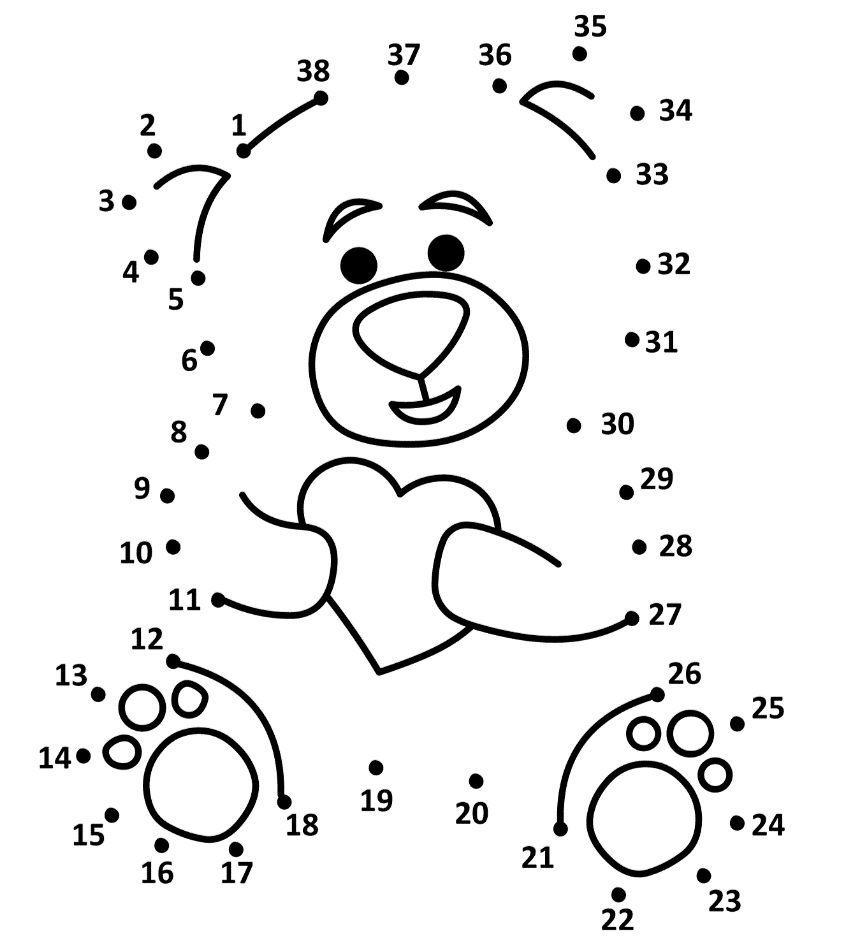
\includegraphics[height=7cm,width=0.48\linewidth,keepaspectratio]{t16_image16.png}\hfill
        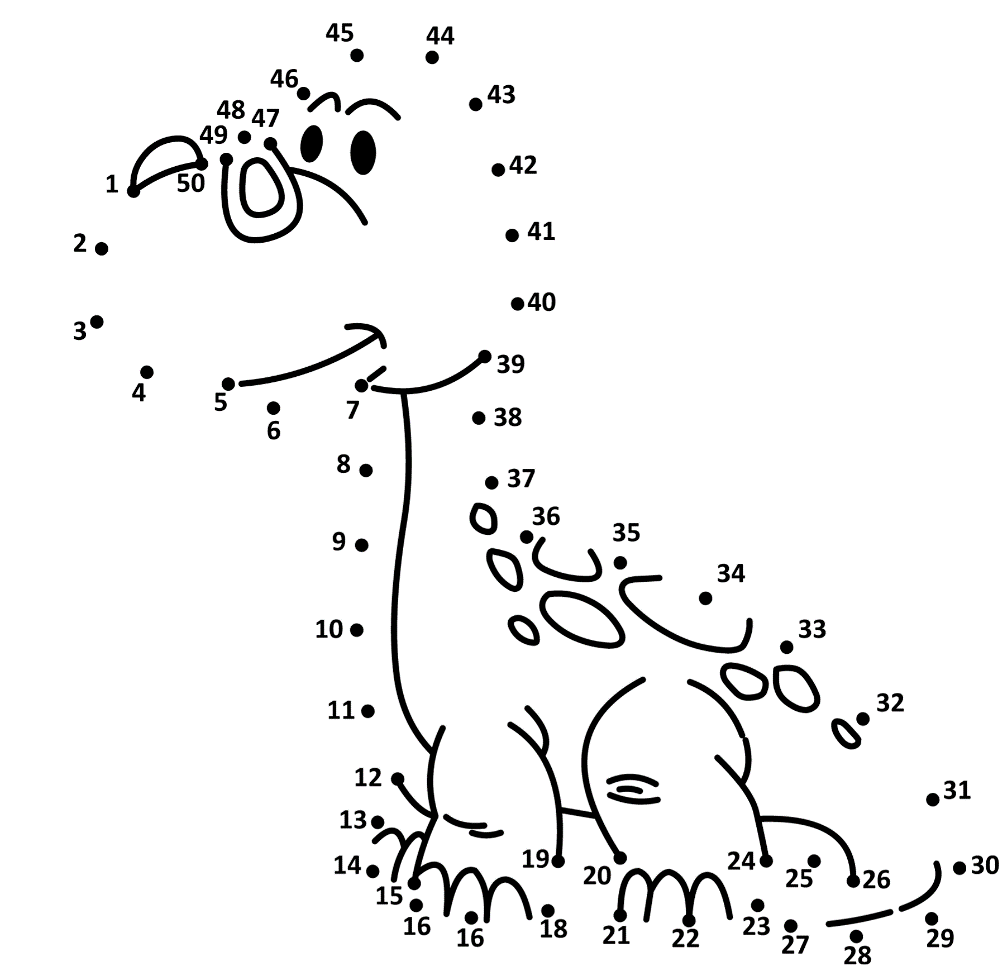
\includegraphics[height=7cm,width=0.48\linewidth,keepaspectratio]{t16_image17.png}\par}
\end{bt}

%%%%%%%%%%%%%%%%%%%%%%%%%%%%%%%%%%%%%%%%%%%%%%%%%%%%%%%%%%
%                       BUỔI 2
%%%%%%%%%%%%%%%%%%%%%%%%%%%%%%%%%%%%%%%%%%%%%%%%%%%%%%%%%%
\newpage
\TTdatlaibai
{\centering
        {\color{mauchinh!120}\bfseries\Large PHIẾU BÀI TẬP TOÁN TƯ DUY CẤP ĐỘ A}\\[3pt]
        {\color{mauchinh!120}\bfseries\Large CHỦ ĐỀ: CÁC SỐ TRONG PHẠM VI 100.\\[2pt] SỐ TRÒN CHỤC (BUỔI 2)}\par}
\vspace{6pt}
\TTthongtin

\begin{bt}
    Đếm theo yêu cầu và điền kết quả.
    \begin{listEX}
        \item Có bao nhiêu chiếc tất? Đếm cách 2.
        \TThinh[4.2cm]{t16_image18.png}
        \item Có bao nhiêu quả? Đếm cách 5.
        \TThinh[4cm]{t16_image19.png}
        \item Có bao nhiêu quả trứng? Đếm cách 10.
        \TThinh[5.5cm]{t16_image20.png}
    \end{listEX}
\end{bt}

\begin{bt}
    Điền số thích hợp vào các toa tàu.
    \TThinh[9cm]{t16_image21.png}
\end{bt}

\begin{bt}
    Thực hiện phép tính.
    \TThinh[7cm]{t16_image25.png}
\end{bt}

\begin{bt}
    Tô màu đỏ vào số chẵn, màu xanh lá vào số lẻ.
    \TThinh[8.5cm]{t16_image26.png}
\end{bt}

\begin{bt}
    Ếch con chỉ nhảy lên những hòn đá ghi số chẵn. Tô màu đường đi giúp ếch con về lá sen.
    \TThinh[7.5cm]{t16_image27.png}
\end{bt}

\begin{bt}
    Điền vào chỗ trống.
    \TThinh[8.5cm]{t16_image28.png}
\end{bt}

\begin{bt}
    Tháp số: số ở mỗi viên gạch bằng tổng hai số ở hai viên gạch ngay bên dưới. Điền số còn thiếu vào các viên gạch trống.
    \TThinh[3.6cm]{t16_image29.png}
\end{bt}

\begin{bt}
    Giải các bài toán sau.
    \begin{listEX}
        \item Lan có 30 nhãn vở, mẹ cho thêm 20 nhãn vở. Hỏi Lan có tất cả bao nhiêu nhãn vở?\\[4pt]
        Phép tính: \TTcham[6cm]
        \item Trên cây có 60 quả cam, bác nông dân hái 40 quả. Hỏi trên cây còn lại bao nhiêu quả cam?\\[4pt]
        Phép tính: \TTcham[6cm]
        \item Mỗi bó có 10 bông hoa. Cô có 5 bó hoa và 4 bông hoa lẻ. Hỏi cô có tất cả bao nhiêu bông hoa?\\[4pt]
        Phép tính: \TTcham[6cm]
        \item Lớp 1A có 3 chục bạn, lớp 1B có 30 bạn. Lớp nào có nhiều bạn hơn?\\[4pt]
        Phép tính: \TTcham[6cm]
    \end{listEX}
\end{bt}

\begin{bt}
    Điền số thích hợp vào ô trống.
    \TThinh[6.5cm]{t16_image30.png}
\end{bt}

\begin{center}
       \faGg\faGg\quad Hết \quad\faGg\faGg
\end{center}
\end{document}
